\documentclass[12pt, a4paper]{article}
\usepackage{pdfpages}
\usepackage{fancyhdr}
\usepackage{listings}
\usepackage{courier}
\usepackage{hyperref}

\pagestyle{fancy}
\fancyhf{}
\fancyhead[L]{Federico del Mazo - 100029}
\fancyhead[R]{01/11/2020}
\renewcommand{\headrulewidth}{0.4pt}
\fancyfoot[C]{\thepage}

\lstset{language=SQL}
\lstset{basicstyle=\footnotesize\ttfamily,breaklines=true}

\begin{document}
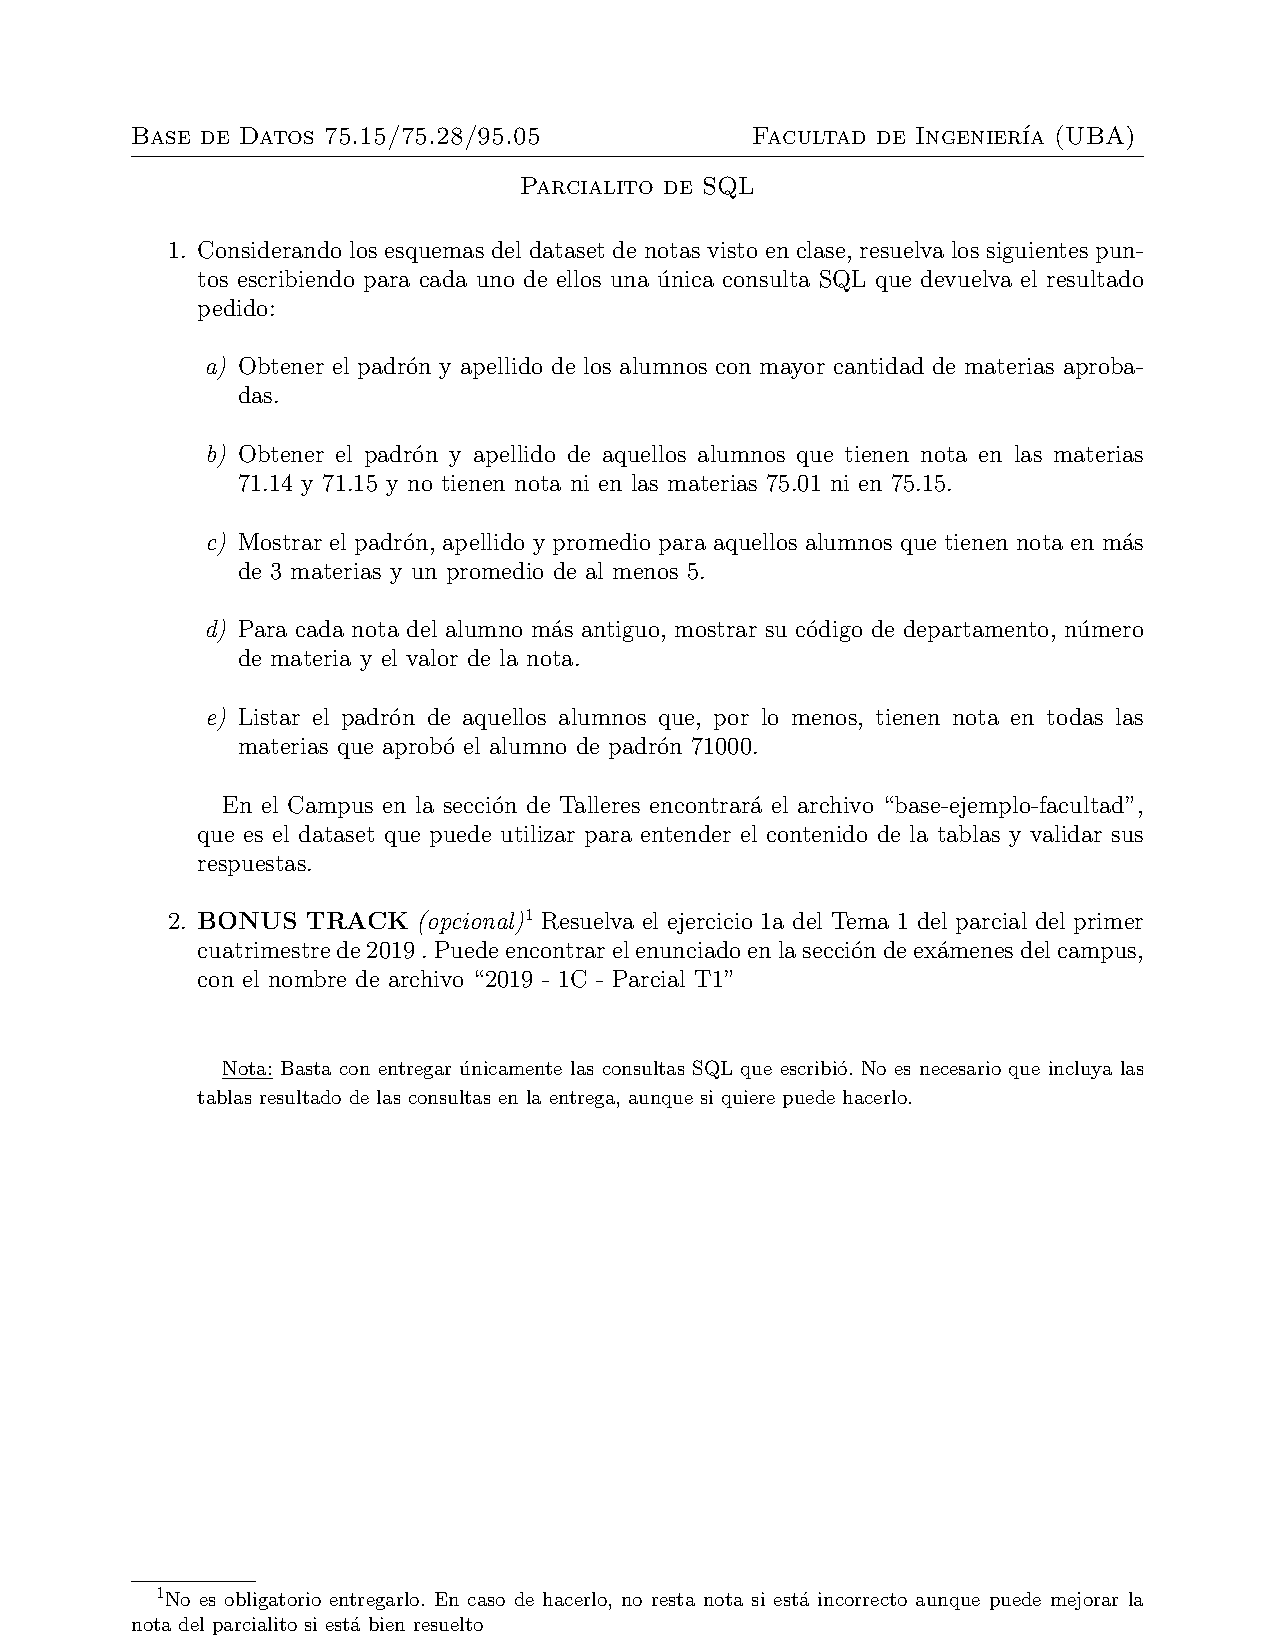
\includepdf{Parcialito4-Enunciado}
\setcounter{page}{1}

\begin{itemize}
\item Obtener el padrón y apellido de los alumnos con mayor cantidad de materias aprobadas.
\begin{lstlisting}[frame=single]
SELECT alumnos.padron, apellido
FROM alumnos
         JOIN notas ON alumnos.padron = notas.padron
WHERE notas.nota >= 4
GROUP BY alumnos.padron
ORDER BY count(*) DESC
LIMIT 1
\end{lstlisting}

Técnicamente, esta query devuelve solo un alumno, por más que puede haber varios que tengan el mayor número de materias aprobadas. Para tener en cuenta estos empates, se puede hacer algo como...

\begin{lstlisting}[frame=single]
SELECT padron, apellido
FROM (
         SELECT alumnos.padron,
                apellido,
                rank() OVER (ORDER BY count(*) DESC) AS rnk
         FROM alumnos
                  JOIN notas ON alumnos.padron = notas.padron
         WHERE notas.nota >= 4
         GROUP BY alumnos.padron
     ) subquery
WHERE rnk <= 1
\end{lstlisting}

\small (Esta mísma idea se puede utilizar en el resto de los ejercicios donde se piden los máximos, como en el ejercicio \textbf{d} donde se necesita encontrar al alumno más antiguo, y este puede ser más de uno, porque se pueden anotar múltiples alumnos en la misma fecha)

\item Obtener el padrón y apellido de aquellos alumnos que tienen nota en las materias 71.14 y 71.15 y no tienen nota ni en las materias 75.01 ni en 75.15.

\begin{lstlisting}[frame=single]
SELECT alumnos.padron, apellido
FROM alumnos
         JOIN notas ON alumnos.padron = notas.padron
WHERE ((codigo = 71 AND numero = 14) OR (codigo = 71 AND numero = 15))
  AND alumnos.padron NOT IN (
    SELECT alumnos.padron
    FROM alumnos
             JOIN notas ON alumnos.padron = notas.padron
    WHERE ((codigo = 75 AND numero = 01) OR (codigo = 75 AND numero = 15))
)
\end{lstlisting}

\item Mostrar el padrón, apellido y promedio para aquellos alumnos que tienen nota en más de 3 materias y un promedio de al menos 5.

\begin{lstlisting}[frame=single]
SELECT alumnos.padron
FROM alumnos
         JOIN notas ON alumnos.padron = notas.padron
GROUP BY alumnos.padron
HAVING (count(alumnos.padron) > 3)
   AND avg(nota) >= 5
\end{lstlisting}

\item Para cada nota del alumno más antiguo, mostrar su código de departamento, número de materia y el valor de la nota.

\begin{lstlisting}[frame=single]
SELECT codigo, numero, nota
FROM notas
WHERE notas.padron IN (
    SELECT padron
    FROM alumnos
    ORDER BY fecha_ingreso ASC
    LIMIT 1
)
\end{lstlisting}

\item Listar el padrón de aquellos alumnos que, por lo menos, tienen nota en todas las materias que aprobó el alumno de padrón 71000.

\begin{lstlisting}[frame=single]
WITH materias AS (
    SELECT codigo, numero
    FROM notas
    WHERE padron = 71000
      AND nota >= 4
)
SELECT padron
FROM (
         SELECT DISTINCT alumnos.padron, codigo, numero
         FROM alumnos
                  JOIN notas ON alumnos.padron = notas.padron
         WHERE (codigo, numero) IN (SELECT codigo, numero FROM materias)
         GROUP BY alumnos.padron, notas.codigo, notas.numero
     ) subquery
GROUP BY padron
HAVING count(*) = (SELECT count(*) FROM materias)
\end{lstlisting}

\end{itemize}

\newpage

Para el ejercicio bonus utilizo la expresion \texttt{SELECT DISTINCT ON}\footnote{\url{https://www.postgresql.org/docs/9.3/sql-select.html\#SQL-DISTINCT}} para quedarme con la fila con la máxima prioridad. Para definir cual es la máxima prioridad, hago uso de \texttt{CASE}: al cruzarme a un mercado, le agregro prioridad 3 a la fila, al cruzarme un local le agrego prioridad 2, y así.

\begin{lstlisting}[frame=single]
SELECT DISTINCT ON (cod_prop) dest.cod_prop,
                              calle,
                              altura,
                              dest.cod_destino,
                              desc_destino,
                              superficie
FROM (
         SELECT cod_prop,
                cod_destino,
                CASE
                    WHEN cod_destino = 9 THEN 3
                    WHEN cod_destino = 5 THEN 2
                    WHEN cod_destino = 15 THEN 1
                    END AS priority
         FROM destinos_por_prop
     ) sq
         INNER JOIN destinos_por_prop dest
                    ON sq.cod_destino = dest.cod_destino
                        AND sq.cod_prop = dest.cod_prop
WHERE priority IS NOT NULL
ORDER BY cod_prop, priority DESC
\end{lstlisting}



\end{document}
